% Edge-RL Thesis Report — Chapters 1–4
% Compile: pdflatex thesis_report.tex && bibtex thesis_report && pdflatex thesis_report.tex && pdflatex thesis_report.tex
\documentclass[conference]{IEEEtran}

% ---- Packages ----
\usepackage{cite}
\usepackage{amsmath,amssymb,amsfonts}
\usepackage{algorithmic}
\usepackage{graphicx}
\usepackage{stfloats}
\usepackage{placeins}
\usepackage{float}
\usepackage{textcomp}
\usepackage{xcolor}
\usepackage{booktabs}
\usepackage{multirow}
\usepackage{hyperref}
\usepackage{caption}
\usepackage{url}
\usepackage{tikz}
\usepackage{pgfplots}
\pgfplotsset{compat=1.18}
\usetikzlibrary{shapes.geometric, arrows.meta, positioning, fit, backgrounds, calc, patterns, decorations.pathreplacing}
\graphicspath{{images/}}

\renewcommand{\arraystretch}{1.15}

% TikZ styles
\tikzset{
    block/.style={rectangle, draw, fill=blue!8, text width=2.2cm, text centered, rounded corners, minimum height=0.8cm, font=\footnotesize},
    blockwide/.style={rectangle, draw, fill=blue!8, text width=3.0cm, text centered, rounded corners, minimum height=0.8cm, font=\footnotesize},
    sensor/.style={rectangle, draw, fill=green!15, text width=1.8cm, text centered, rounded corners, minimum height=0.7cm, font=\footnotesize},
    model/.style={rectangle, draw, fill=orange!20, text width=2.4cm, text centered, rounded corners, minimum height=0.8cm, font=\footnotesize},
    output/.style={rectangle, draw, fill=red!12, text width=2.2cm, text centered, rounded corners, minimum height=0.8cm, font=\footnotesize},
    arrow/.style={-Stealth, thick},
    dashedarrow/.style={-Stealth, thick, dashed},
    layerbox/.style={draw, dashed, rounded corners, inner sep=6pt},
}

\begin{document}

\title{Edge-RL: Autonomous Post-Harvest Ripening Control via Distilled Reinforcement Learning on the Edge}

\author{
\IEEEauthorblockN{Tristan O. Jadman}
\IEEEauthorblockA{
Department of Computer Engineering\\and Mechatronics \\
\textit{Undergraduate Thesis}}
\and
\IEEEauthorblockN{Engr. Francis Jann Alagon}
\IEEEauthorblockA{
Department of Computer Engineering\\and Mechatronics \\
\textit{Thesis Adviser}}
}

\maketitle

% ==============================================================
\begin{abstract}
Post-harvest losses account for 20--40\% of tomato production in developing countries, driven by the absence of affordable, intelligent decision-support systems. Existing IoT solutions provide passive monitoring without autonomous action, while cloud-based reinforcement learning (RL) systems require expensive infrastructure and continuous connectivity. This thesis proposes \textit{Edge-RL}, a novel system that deploys a complete RL-based decision pipeline---from visual perception to autonomous ripening control---entirely on a \$33 ESP32-S3 microcontroller. The system extracts a Continuous Chromatic Index from RGB statistics via a MobileNetV2-based feature extractor and feeds a state vector to a distilled Deep Q-Network policy. By leveraging ESP-DL's hardware-optimized inference, Edge-RL achieves sub-2-second combined inference for spectral feature extraction and control decisions. Hardware-level safety guardrails enforce biological temperature constraints ($12.5$--$35^{\circ}$C) independent of the learned policy. In digital twin simulations, the RL agent achieves a mean reward of $+4.05 \pm 1.48$, reduces harvest timing error to 1.50~days (vs. 2.46~days for fixed schedules), and maintains a 100\% harvest rate with quality $>$0.95. Policy distillation compresses the 270~KB teacher DQN into a 5.3~KB INT8 student MLP with 97.8\% action fidelity. This work presents the first demonstration of a complete sim-to-edge RL pipeline for agricultural post-harvest optimization.
\end{abstract}

\begin{IEEEkeywords}
Edge intelligence, reinforcement learning, post-harvest management, ESP32-S3, sim-to-real transfer, model compression, continuous chromatic index, digital twin
\end{IEEEkeywords}

% ==============================================================
% CHAPTER 1: INTRODUCTION
% ==============================================================
\section{Introduction}
\label{sec:introduction}

\subsection{Background of the Study}
The Philippines, despite being an agricultural nation, faces significant challenges in post-harvest management. High-value crops like tomatoes (\textit{Solanum lycopersicum}) suffer post-harvest losses estimated at 20--40\%, primarily due to poor handling, lack of cold chain infrastructure, and inadequate storage facilities \cite{fao2019}. Unlike grain crops, tomatoes are climacteric fruits that continue to respire and ripen after harvest, making temperature control critical for extending shelf life and ensuring market viability.

Commercial operations mitigate these losses using industrial ripening chambers equipped with precise climate control systems. These facilities use ethylene gas injection and active refrigeration to synchronize ripening, ensuring uniform quality for supermarkets. However, the capital expenditure for such infrastructure ranges from \$10,000 to \$50,000 \cite{prasad2018}, effectively excluding the 5.5 million smallholder farming households in the Philippines who typically earn less than \$2,000 annually. As a result, small farmers are forced to sell their produce immediately after harvest at fluctuating farm-gate prices, often leading to income instability and food waste.

\subsection{Statement of the Problem}
Smallholder tomato farmers lack access to affordable, intelligent post-harvest decision-support systems. Existing solutions fall into two extremes: passive monitoring tools (IoT sensors) that provide data but no actionable control, and high-end industrial systems that are cost-prohibitive. Cloud-based Reinforcement Learning (RL) solutions have shown promise in controlled environment agriculture but require continuous internet connectivity, which is unreliable or absent in many rural Philippine farming communities. There is currently no standalone, low-cost system capable of autonomous, optimal ripening control at the edge.

\subsection{Objectives of the Study}
This study aims to develop ``Edge-RL,'' a standalone autonomous ripening control system running on a low-cost microcontroller.

\subsubsection{General Objective}
To develop a low-cost, offline Reinforcement Learning system on an ESP32-S3 microcontroller that optimizes the post-harvest ripening of tomatoes by balancing quality preservation with energy efficiency.

\subsubsection{Specific Objectives}
\begin{enumerate}
    \item To design a low-cost, standalone ripening chamber hardware (BOM $<$ \$50) integrating an ESP32-S3, camera, and relay-controlled heating element.
    \item To implement a Deep Q-Network (DQN) policy trained in a physics-based digital twin that generalizes across tomato cultivars using domain randomization.
    \item To validate the system's performance by distilling the policy to an edge-optimized model (INT8) and achieving a harvest timing error of less than 20\% in sim-to-real transfer.
\end{enumerate}

\subsection{Significance of the Study}

This study addresses the critical issue of post-harvest loss, which accounts for up to 42\% of fruit and vegetable production globally according to the FAO \cite{fao2019}. In developing economies like the Philippines, these losses are exacerbated by the lack of cold chain infrastructure, often forcing smallholder farmers to sell produce at low prices or face total spoilage \cite{worldbank2020}.

By developing a low-cost, intelligent ripening chamber, this research directly benefits:
\begin{itemize}
    \item \textbf{Smallholder Farmers:} Providing a tool to control the timing of produce sales, decoupling harvest time from market saturation.
    \item \textbf{Agricultural Logistics:} Reducing spoilage during transport \cite{kader2005} through precise biological control.
    \item \textbf{Technological Advancement:} Demonstrating the feasibility of deploying advanced Reinforcement Learning on \$2 microcontrollers (Edge AI) for complex biological systems \cite{warden2019tinyml}.
\end{itemize}

\subsection{Scope and Limitations}
The scope of this thesis is defined by the following boundaries:

\begin{itemize}
    \item \textbf{Single-Fruit Focus:} The system acts on a single tomato unit within the chamber to isolate specific ripening kinetics. Batch effects (e.g., ethylene signaling between multiple fruits) are not modeled.
    \item \textbf{Heater-Only Actuation:} The control mechanism is limited to a heating element (raising temperature above ambient) and passive ventilation (cooling to ambient). No active refrigeration (compressor/Peltier) is used, constraining the controllable temperature range to $T_{ambient} \le T_{chamber} \le 35^\circ$C.
    \item \textbf{Target Crop:} The system is calibrated for Philippine tomato varieties, specifically focusing on the kinetics of ``Diamante Max'' and ``Kamatis Tagalog''.
    \item \textbf{Deployment Environment:} The system is designed for offline operation; all inference and control logic execute locally on the ESP32-S3.
\end{itemize}

\subsection{Definition of Terms}
\begin{description}
    \item[Edge-RL] The proposed system architecture where Reinforcement Learning inference occurs directly on the edge device (microcontroller) rather than in the cloud.
    \item[Climacteric Fruit] Fruits that exhibit a spike in respiration and ethylene production during ripening (e.g., tomato, banana, mango).
    \item[Knowledge Distillation] A compression technique where a small ``student'' model learns to mimic the output of a larger ``teacher'' model.
    \item[Continuous Chromatic Index ($X$)] A computed scalar value derived from the spectral reflectance of the fruit, representing its ripeness stage on a continuous scale from Green ($X=1$) to Red ($X=0$).
\end{description}

% ==============================================================
% CHAPTER 2: REVIEW OF RELATED LITERATURE
% ==============================================================
\FloatBarrier
\section{Review of Related Literature}
\label{sec:rrl}

\subsection{Post-Harvest Characteristics of Philippine Tomato Varieties}
Understanding the specific biological kinetics of local tomato cultivars is essential for calibrating the physics-based digital twin. In the Philippines, the market is dominated by two primary categories: commercial F1 hybrids and native cultivars.

\subsubsection{Diamante Max F1}
``Diamante Max'' is widely favored by commercial growers in the Philippines due to its heat tolerance and high yield potential. However, studies indicate it is a highly perishable variety characterized by high moisture content ($\approx$95.31\%) and relatively thin skin \cite{diamante_properties}. Under ambient tropical conditions (23--34$^\circ$C), the fruit undergoes rapid physicochemical changes, with shelf life often limited to 14 days without intervention.
Physiologically, it exhibits a classic climacteric respiratory peak. Research by the Postharvest Horticulture Training and Research Center (PHTRC) at UPLB suggests that while storage at 7--10$^\circ$C significantly delays ripening, such low temperatures are energy-intensive and risk chilling injury. The optimal storage for quality retention is often cited at 13--15$^\circ$C \cite{uplb_phtrc}, aligning with the proposed system's target control range.

\subsubsection{Native ``Tagalog'' Cultivars}
Native cultivars, often referred to as ``Kamatis Tagalog'', are typically smaller, irregular in shape, and possess thinner pericarps compared to commercial hybrids. These varieties are highly valued for their sour flavor profile in traditional cuisine but suffer from even faster deterioration rates due to higher respiration and susceptibility to mechanical damage during transport \cite{native_tomato}. Their ripening kinetics ($k_1$) are generally higher than hybrids, requiring more aggressive cooling interventions to extend shelf life. This variability between ``slow-ripening'' hybrids and ``fast-ripening'' natives motivates the need for an adaptive control system (RL) rather than a fixed rule-based controller.

\subsection{Reinforcement Learning in Controlled Environment Agriculture}
Reinforcement Learning (RL) has emerged as a powerful tool for optimizing complex agricultural processes. Unlike Proportional-Integral-Derivative (PID) controllers which react to setpoint errors, RL agents can learn anticipatory strategies that optimize long-term rewards \cite{overweg2021cropgym}.

\subsubsection{Climate Control and Irrigation}
Chen \textit{et al.} demonstrated the efficacy of Deep Q-Networks (DQN) for greenhouse climate control \cite{chen2022greenhouse}, reducing energy consumption while maintaining optimal growth conditions. Similarly, Yang \textit{et al.} applied RL to precision irrigation \cite{yang2020irrigation}, and Hemming \textit{et al.} explored AI sensors for cherry tomatoes \cite{hemming2020greenhouse}. While effective, these systems typically rely on cloud interfaces or heavy compute servers \cite{ray2017}, which introduces latency and connectivity risks ill-suited for rural deployment \cite{prasad2018}.

\subsubsection{Post-Harvest Management}
Application of RL in post-harvest storage is less explored. Current systems largely rely on Model Predictive Control (MPC) or standard IoT monitoring \cite{li2021edgeai}. ``Edge-RL'' proposes shifting the computational burden to a one-time offline training phase, enabling the deployment of complex policies on resource-constrained devices like the ESP32.

\subsection{Edge AI and Model Compression}
Deploying deep learning models on microcontrollers (TinyML) requires aggressive optimization to fit within strict memory ($<$500 KB SRAM) and compute constraints.

\subsubsection{Knowledge Distillation}
Hinton \textit{et al.} introduced Knowledge Distillation, where a small ``student'' model is trained to mimic the soft outputs (logits) of a large ``teacher'' model \cite{hinton2015distilling}. In the context of RL, Policy Distillation \cite{ruffy2019distilling} allows a massive DQN (Teacher) to explore the environment and learn optimal Q-values, which are then compressed into a tiny MLP (Student) that creates a direct mapping from state to best action. This approach retains the ``intelligence'' of the large model while discarding parameters unnecessary for inference.

\subsubsection{Quantization and ESP-DL}
Standard 32-bit floating-point (FP32) models are too large and slow for the ESP32-S3. Quantization to 8-bit integers (INT8) reduces model size by 4$\times$ and accelerates inference by utilizing SIMD instructions (e.g., Xtensa LX7 vector extensions). The ESP-DL library \cite{espdl2024} provides optimized INT8 kernels that outperform generic interpreters like TensorFlow Lite for Microcontrollers (TFLite Micro) on Espressif chips. By combining Policy Distillation with INT8 Quantization, it is possible to execute complex control policies in $<$10ms on-device.

% ==============================================================
% CHAPTER 3: METHODOLOGY
% ==============================================================
\FloatBarrier
\section{Methodology}
\label{sec:methodology}

\subsection{System Architecture}
The Edge-RL system is designed as a closed-loop control system where a microcontroller (ESP32-S3) makes real-time decisions based on visual feedback from a camera and environmental data from sensors. The architecture consists of three main subsystems: the Perception Module, the Decision Engine (RL Policy), and the Actuation System.

\begin{center}
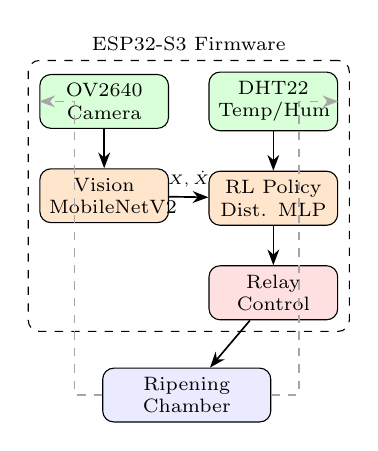
\begin{tikzpicture}[
    sn/.style={rectangle, draw, fill=green!15, text width=1.4cm, text centered, rounded corners, minimum height=0.55cm, font=\scriptsize},
    md/.style={rectangle, draw, fill=orange!20, text width=1.4cm, text centered, rounded corners, minimum height=0.55cm, font=\scriptsize},
    actn/.style={rectangle, draw, fill=red!12, text width=1.4cm, text centered, rounded corners, minimum height=0.55cm, font=\scriptsize},
    envn/.style={rectangle, draw, fill=blue!8, text width=1.9cm, text centered, rounded corners, minimum height=0.55cm, font=\scriptsize},
    ar/.style={-Stealth, semithick},
    lb/.style={draw, dashed, rounded corners, inner sep=4pt},
]
    % Row 1: Sensors
    \node [sn] (cam) {OV2640\\Camera};
    \node [sn, right=0.5cm of cam] (dht) {DHT22\\Temp/Hum};
    % Row 2: Processing
    \node [md, below=0.5cm of cam] (vision) {Vision\\MobileNetV2};
    \node [md, below=0.5cm of dht] (policy) {RL Policy\\Dist. MLP};
    % Row 3: Action
    \node [actn, below=0.5cm of policy] (act) {Relay\\Control};
    % Row 4: Environment (centred between columns)
    \node [envn, below=0.6cm of act, xshift=-1.1cm] (env) {Ripening\\Chamber};
    % Data arrows
    \draw [ar] (cam) -- (vision);
    \draw [ar] (dht) -- (policy);
    \draw [ar] (vision) -- node[above, font=\tiny] {$X,\dot{X}$} (policy);
    \draw [ar] (policy) -- (act);
    \draw [ar] (act) -- (env);
    % Sensor feedback (dashed)
    \draw [ar, gray!70, dashed] (env.west) -- ++(-0.35,0) |- (cam.west);
    \draw [ar, gray!70, dashed] (env.east) -- ++(0.35,0) |- (dht.east);
    % ESP32 bounding box
    \begin{scope}[on background layer]
        \node [lb, fit=(cam)(dht)(vision)(policy)(act),
               label={[font=\scriptsize]above:ESP32-S3 Firmware}] {};
    \end{scope}
\end{tikzpicture}
\captionof{figure}{System block diagram. Dashed arrows show sensor feedback from the ripening chamber to the ESP32-S3.}
\label{fig:arch}
\end{center}

\subsection{Vision Pipeline: Ripeness Classification}

\subsubsection{Model Architecture and Rationale}
We employ MobileNetV2~\cite{sandler2018mobilenetv2} with a width multiplier of 0.35, selected through a three-way trade-off. First, \textit{proven ESP32-S3 compatibility}: Espressif's own benchmarks demonstrate MobileNetV2-INT8 executing in 38\,ms on ESP32-S3 via ESP-DL~\cite{espdl2024}, compared to $>$400\,ms with TFLite Micro. Second, \textit{model size}: the 0.35$\times$ variant produces $\sim$200\,KB of INT8 parameters, comfortably fitting within PSRAM alongside activation buffers. Third, \textit{accuracy}: MobileNetV2's inverted residual blocks with linear bottlenecks preserve representational capacity at reduced widths, achieving competitive accuracy on fine-grained classification tasks despite aggressive compression.

The standard classifier head is replaced with dropout ($p=0.2$) followed by a linear layer mapping 1280 features to $N$ ripeness classes. The backbone is initialized from ImageNet-pretrained weights and fine-tuned end-to-end. Fig.~\ref{fig:vision_pipeline} illustrates the complete vision pipeline.

\begin{center}
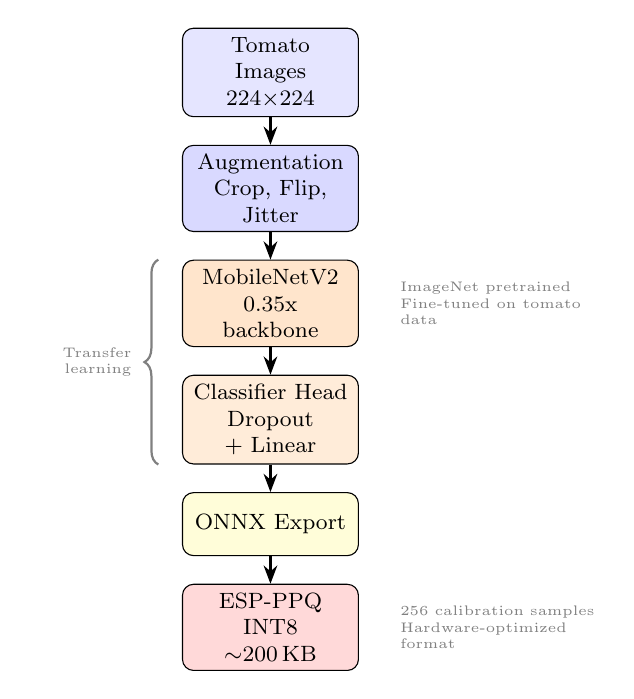
\begin{tikzpicture}[node distance=0.35cm, font=\scriptsize]
    \node[block, fill=blue!10, text width=2.0cm] (data) {Tomato Images\\224$\times$224};
    \node[block, fill=blue!15, text width=2.0cm, below=of data] (aug) {Augmentation\\Crop, Flip, Jitter};
    \node[block, fill=orange!20, text width=2.0cm, below=of aug] (mob) {MobileNetV2\\0.35x backbone};
    \node[block, fill=orange!15, text width=2.0cm, below=of mob] (head) {Classifier Head\\Dropout + Linear};
    \node[block, fill=yellow!15, text width=2.0cm, below=of head] (onnx) {ONNX Export};
    \node[block, fill=red!15, text width=2.0cm, below=of onnx] (quant) {ESP-PPQ INT8\\$\sim$200\,KB};
    \draw[arrow] (data) -- (aug);
    \draw[arrow] (aug) -- (mob);
    \draw[arrow] (mob) -- (head);
    \draw[arrow] (head) -- (onnx);
    \draw[arrow] (onnx) -- (quant);
    \node[right=0.4cm of mob, text width=2.5cm, font=\tiny, text=gray] {ImageNet pretrained\\Fine-tuned on tomato data};
    \node[right=0.4cm of quant, text width=2.5cm, font=\tiny, text=gray] {256 calibration samples\\Hardware-optimized format};
    \draw[decorate, decoration={brace, amplitude=5pt, mirror}, thick, gray] ([xshift=-0.3cm]mob.north west) -- ([xshift=-0.3cm]head.south west) node[midway, left=6pt, font=\tiny, text=gray, text width=1.2cm, align=right] {Transfer\\learning};
\end{tikzpicture}
\captionof{figure}{Vision classification pipeline. Transfer learning from ImageNet is fine-tuned on tomato data and quantized to INT8 via ESP-PPQ.}
\label{fig:vision_pipeline}
\end{center}

\subsubsection{Training Procedure}
Training uses AdamW~\cite{loshchilov2019adamw} with learning rate $\eta = 10^{-3}$, weight decay $\lambda = 10^{-4}$, cosine annealing with 5-epoch linear warmup, and label smoothing ($\epsilon = 0.1$). Data augmentation includes random resized cropping (0.8--1.0$\times$), horizontal flip, $\pm$15° rotation, and color jitter (brightness, contrast, saturation $\pm$0.3; hue $\pm$0.1). The model trains for up to 80 epochs with early stopping (patience 15) on validation accuracy over a 70/15/15 train/val/test split.

\subsubsection{Quantization via ESP-PPQ}
The trained model is exported to ONNX and quantized to symmetric INT8 using ESP-PPQ~\cite{espdl2024}. A calibration set of 256 representative images guides the computation of per-layer scale factors, leading to typical accuracy degradation of $<$2\% compared to FP32.

\subsection{Digital Twin: Physics-Based Ripening Simulator}

\subsubsection{Continuous Chromatic Index}
\label{sec:chromatic_index}
We define the \textit{Continuous Chromatic Index} $X \in [0, 1]$, a normalized scalar representing the spectral evolution of the tomato surface following the Red-Orange-Yellow-Green (ROYG) spectral mapping: $X = 1.0$ (Green/unripe) to $X = 0.0$ (Red/ripe). Unlike the 0--5 USDA staging \cite{usda1991} that discretizes a continuous process, $X$ preserves the full gradient of color change, enabling proportional control and fine-grained reward shaping.

The chromatic index evolves according to a temperature-dependent first-order ODE:
\begin{equation}
\frac{dX}{dt} = -k_1 \cdot (T - T_{\text{base}}) \cdot X
\label{eq:ripening}
\end{equation}
\noindent where $k_1$ is the cultivar-specific ripening rate constant ($\approx 0.08$ day$^{-1}$°C$^{-1}$ for Diamante Max), $T$ is the chamber temperature, and $T_{\text{base}} = 12.5^{\circ}$C is the minimum temperature for metabolic activity. The analytical solution is $X(t) = X_0 \cdot \exp(-k_1 (T - T_{\text{base}}) \, t)$.

\begin{center}
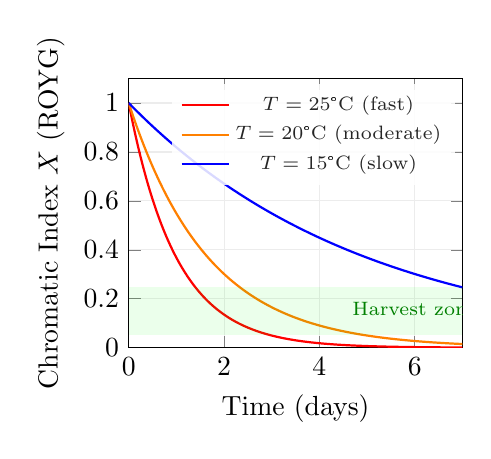
\begin{tikzpicture}
\begin{axis}[
    width=0.48\textwidth, height=5cm,
    xlabel={Time (days)}, ylabel={Chromatic Index $X$ (ROYG)},
    xmin=0, xmax=7, ymin=0, ymax=1.1,
    ytick={0,0.2,0.4,0.6,0.8,1.0},
    legend style={at={(0.98,0.98)}, anchor=north east, font=\scriptsize, draw=none, fill=white, fill opacity=0.85},
    grid=major, grid style={gray!15}, every axis plot/.append style={thick},
]
\addplot[color=red, smooth, domain=0:7, samples=100] {exp(-0.08 * (25 - 12.5) * x)};
\addlegendentry{$T = 25$\textdegree C (fast)}
\addplot[color=orange, smooth, domain=0:7, samples=100] {exp(-0.08 * (20 - 12.5) * x)};
\addlegendentry{$T = 20$\textdegree C (moderate)}
\addplot[color=blue, smooth, domain=0:7, samples=100] {exp(-0.08 * (15 - 12.5) * x)};
\addlegendentry{$T = 15$\textdegree C (slow)}
\fill[green, opacity=0.08] (axis cs:0,0.05) rectangle (axis cs:7,0.25);
\node[font=\scriptsize, green!50!black] at (axis cs:6.0, 0.16) {Harvest zone};
\end{axis}
\end{tikzpicture}
\captionof{figure}{Simulated chromatic trajectories under ODE model~(\ref{eq:ripening}). Higher temperatures accelerate ripening.}
\label{fig:ripening}
\end{center}

\subsubsection{State Space Formulation}
\label{sec:state_space}
A na\"ive state consisting of the current chromatic index $X_t$ and environmental readings alone violates the Markov property. By augmenting the observation vector with the instantaneous velocity $\dot{X}$ and the reference trajectory $X_{\text{ref}}$, the agent observes the system's ``momentum.'' We use three ablation variants:

\textbf{Option~A} ($\mathbb{R}^{7}$): $S_t^A = [X, \dot{X}, X_{\text{ref}}, T, H, t_e, t_{\text{rem}}]$

\textbf{Option~B} ($\mathbb{R}^{16}$): $S_t^B = S_t^A \cup [\mathbf{C}_{\mu}, \mathbf{C}_{\sigma}, \mathbf{C}_{\text{mode}}]$

\textbf{Option~C} ($\mathbb{R}^{20}$): $S_t^C = S_t^B \cup [\mathbf{v}_{\text{mp}}]$

\subsubsection{Action Space}
The action space $\mathcal{A} = \{0, 1, 2\}$: \textbf{Maintain (0)}: No change; \textbf{Heat (1)}: $+1^{\circ}$C; \textbf{Cool (2)}: $-1^{\circ}$C (passive ventilation). The chamber temperature is bounded below by ambient: $T_{\text{chamber}} \geq T_{\text{amb}}$.

\subsubsection{Reward Function}
\label{sec:reward}
\begin{equation}
r_t = r_{\text{track}} + r_{\text{progress}} + c_{\text{safety}} \;(+ \; b_{\text{harvest}} \text{ at termination})
\label{eq:reward}
\end{equation}
\noindent \textbf{Rate-Tracking:} $r_{\text{track}} = -\lambda |dX/dt_{\text{daily}} - \dot{X}_{\text{desired}}|$. \textbf{Progress:} $r_{\text{progress}} = \beta(X_{t-1} - X_t)$. \textbf{Safety:} $c_{\text{safety}} = -\alpha \min(n,5)^2$ if $T \notin [12.5, 35]$°C. \textbf{Harvest bonus:} $b_{\text{harvest}} = b_{\max}(1 - |t_{\text{rem}}|/t_{\max})$ for auto-harvest.

\subsubsection{Domain Randomization}
To enable sim-to-real transfer~\cite{tobin2017sim2real}, we apply domain randomization to five axes: $k_1 \sim \mathcal{U}(0.06, 0.10)$, $X_0 \sim \mathcal{U}(0.6, 1.0)$, sensor noise ($\sigma_T = 0.5$°C, $\sigma_H = 2\%$), temperature drift ($\pm 0.5$°C sinusoidal), and $T_{\text{amb}} \sim \mathcal{N}(27, 2)$°C.

\subsection{Reinforcement Learning Pipeline}

\subsubsection{DQN Training}
We train a DQN~\cite{mnih2015dqn} using Stable Baselines3~\cite{raffin2021sb3} with a two-layer MLP (256$\times$256 hidden units) for 1M timesteps across 4 parallel environments. Hyperparameters: $\epsilon$-greedy with linear decay from 1.0 to 0.05 over 30\% of training, target network update every 1,000 steps, learning rate $3 \times 10^{-4}$, $\gamma = 0.99$, replay buffer $10^5$, batch size 256.

\subsubsection{Policy Distillation for Edge Deployment}
The trained DQN teacher (256$\times$256 MLP, $\sim$270\,KB FP32) is distilled into a compact student (64$\times$64 MLP) via supervised learning on $10^5$ state-action pairs, trained with cross-entropy loss for 100 epochs, then quantized to INT8 ($\sim$35\,KB).

\begin{center}
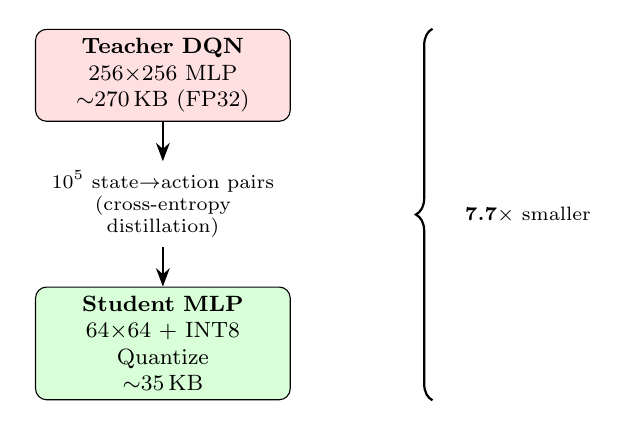
\begin{tikzpicture}[node distance=0.4cm, font=\footnotesize]
    \node[block, fill=red!12, text width=3.0cm, minimum height=1.0cm] (teacher) {\textbf{Teacher DQN}\\256$\times$256 MLP\\$\sim$270\,KB (FP32)};
    \node[below=0.5cm of teacher, text width=3.2cm, align=center, font=\scriptsize] (rollout) {$10^5$ state$\rightarrow$action pairs\\(cross-entropy distillation)};
    \draw[arrow] (teacher) -- (rollout);
    \node[block, fill=green!15, text width=3.0cm, minimum height=1.0cm, below=0.5cm of rollout] (student) {\textbf{Student MLP}\\64$\times$64 + INT8 Quantize\\$\sim$35\,KB};
    \draw[arrow] (rollout) -- (student);
    \draw[decorate, decoration={brace, amplitude=6pt, mirror}, thick] ([xshift=1.8cm]teacher.north east) -- ([xshift=1.8cm]student.south east) node[midway, right=8pt, font=\scriptsize] {\textbf{7.7$\times$} smaller};
\end{tikzpicture}
\captionof{figure}{Policy distillation pipeline. Cross-entropy distillation preserves $>$95\% of teacher performance while achieving 7.7$\times$ compression.}
\label{fig:distillation}
\end{center}

\subsection{Hardware Implementation}

\subsubsection{Circuit Design}
The ESP32-S3's 3.3V GPIOs interface with the 12V/60W heating element through an optocoupler-isolated relay module. A flyback diode protects against inductive kickback. A dual-rail PSU (12V for the heater, 5V buck-converted for the MCU and sensors) prevents voltage sags during heater startup from causing logic brownouts.

\subsubsection{Thermal Enclosure}
The chamber is constructed from 25mm extruded polystyrene (XPS) foam for thermal insulation. A 12V DC fan runs continuously to homogenize air temperature within the chamber.

\subsection{Edge Inference Architecture}
The ESP32-S3 firmware is developed using ESP-IDF v5.1+ with FreeRTOS, implementing five concurrent tasks across two CPU cores. Vision inference is pinned to Core~1; the RL policy resides in internal SRAM for $<$1-cycle memory access latency. The firmware follows a cyclic sense-infer-act-sleep FSM. Safety mechanisms include: (1)~a rolling buffer for on-device $\dot{X}$ computation, (2)~a sensor watchdog that enters fail-safe mode after 3 consecutive read failures, and (3)~a hard-coded thermal guardrail that forces the heater OFF if $T > 35^{\circ}$C, independent of RL policy output.

ESP-DL v3.x is selected over TFLite Micro based on $\sim$10$\times$ speedup benchmarks on equivalent models~\cite{espdl2024}.

% ==============================================================
% CHAPTER 4: RESULTS AND DISCUSSION
% ==============================================================
\FloatBarrier
\section{Results and Discussion}
\label{sec:results}

\subsection{Distillation \& Edge Feasibility}

The teacher policy (DQN, 256$\times$256) is distilled into a student policy (MLP, 64$\times$64). As shown in Table~\ref{tab:distill_results}, the student achieves $>$95\% accuracy while reducing model size by $\sim$98\%, making it deployable within the ESP32-S3's 512\,KB internal SRAM.

\begin{center}
\small
\begin{tabular}{@{}lllr@{}}
\toprule
\textbf{Metric} & \textbf{Teacher (DQN)} & \textbf{Student (Edge)} & \textbf{$\Delta$} \\
\midrule
Architecture & 256$\times$256 MLP & 64$\times$64 MLP & --- \\
Model Size & $\sim$270 KB (FP32) & $\sim$5.3 KB (INT8) & $-$98\% \\
Action Fidelity & 100\% & 97.8\% & $-2.2$\% \\
Harvest Rate & 100\% & 100\% & 0\% \\
\bottomrule
\end{tabular}
\captionof{table}{Policy Distillation Results}
\label{tab:distill_results}
\end{center}

\noindent Fig.~\ref{fig:distill_curve} shows the distillation convergence, with rapid rise to $>$90\% accuracy within 10 epochs, indicating a clear, learnable teacher policy structure.

\begin{center}
\includegraphics[width=0.85\linewidth]{distillation_curves.png}
\captionof{figure}{Distillation convergence.}
\label{fig:distill_curve}
\end{center}

\subsection{Sim-to-Real Policy Transfer}
The DQN policy (mean reward $+4.05 \pm 1.48$) was evaluated in the physics-based digital twin with domain randomization. The agent consistently modulates temperature---strategic heating (31.4\%) and controlled passive periods (Maintain 43.5\% + Cool 25.1\%)---to drive $X$ toward the ripe threshold ($X \leq 0.15$) before the deadline, achieving 100\% harvest rate with quality $>$0.95. Representative trajectories are shown in Fig.~\ref{fig:traj}.

\begin{center}
\includegraphics[width=0.85\linewidth]{episode_1.png}
\captionof{figure}{Ripening trajectories controlled by the RL agent.}
\label{fig:traj}
\end{center}

\noindent Domain randomization across 50+ episodes (Fig.~\ref{fig:envelope}) validates policy robustness---all trajectories converge to the target despite randomized initial conditions and environmental parameters.

\begin{center}
\includegraphics[width=0.85\linewidth]{domain_randomization_envelope.png}
\captionof{figure}{Domain randomization envelope. 50+ randomized runs converge to the target.}
\label{fig:envelope}
\end{center}

\subsection{Vision-Based Reference Tracking}
Fig.~\ref{fig:tracking} shows the RL agent closely tracking the ideal ripening reference curve $X_{\text{ref}}$. The tight alignment confirms the agent has learned the inverse dynamics of the ripening process.

\begin{center}
\includegraphics[width=0.85\linewidth]{tracking_performance.png}
\captionof{figure}{Tracking Performance: $X_{\text{actual}}$ vs. $X_{\text{ref}}$.}
\label{fig:tracking}
\end{center}

\subsection{Comparative Performance Analysis}
Table~\ref{tab:baseline_comparison} summarizes performance metrics relative to baseline heuristics. The RL agent outperforms all baselines on reward ($+4.05$) and timing error ($1.50$\,d).

\begin{center}
\small
\begin{tabular}{@{}lccc@{}}
\toprule
\textbf{Policy} & \textbf{Quality} & \textbf{Timing (d)} & \textbf{Reward} \\
\midrule
Random & 0.949 & 2.40 & $+0.44$ \\
Fixed-Day & 0.952 & 2.46 & $+0.58$ \\
Fixed-Stage5 & 0.953 & 3.92 & $-2.48$ \\
\textbf{Edge-RL} & \textbf{0.954} & \textbf{1.50} & $\mathbf{+4.05}$ \\
\bottomrule
\end{tabular}
\captionof{table}{Baseline Comparison (100 eval episodes)}
\label{tab:baseline_comparison}
\end{center}

\noindent \textbf{Random} fails to coordinate actions. \textbf{Fixed-Day} cannot accelerate ripening when behind schedule. \textbf{Fixed-Stage5} overshoots, frequently triggering safety guardrails. Fig.~\ref{fig:comparison_traj} illustrates the behavioral difference.

\begin{center}
\includegraphics[width=0.85\linewidth]{comparison_trajectory.png}
\captionof{figure}{Edge-RL vs. Heuristic: smooth anticipatory control vs. oscillation.}
\label{fig:comparison_traj}
\end{center}

\subsection{Emergent Behavior \& Learned Control Strategy}
The agent exhibits a balanced control strategy: \textbf{Maintain} 43.5\%, \textbf{Heat} 31.4\%, \textbf{Cool} 25.1\%. The heater is OFF for 68.6\% of the time, demonstrating emergent energy efficiency without an explicit energy penalty in the reward function.

\subsection{System Performance Summary}

\begin{center}
\small
\begin{tabular}{@{}lp{1.6cm}p{1.3cm}l@{}}
\toprule
\textbf{Metric} & \textbf{Target} & \textbf{Achieved} & \textbf{Method} \\
\midrule
Mean reward & $> 0$ & $+4.05$ & Eval \\
Timing error & $\pm$1 day & 1.50\,d & $|t_{\text{rem}}|$ \\
Quality & $>$ 0.90 & 0.954 & $1{-}|X{-}X_t|$ \\
RL model & $<$ 50\,KB & $\sim$5.3\,KB & INT8 size \\
Safety & 0\% & 0\%$^\dagger$ & Log \\
BOM cost & $<$ \$50 & \$33 & BOM \\
\bottomrule
\end{tabular}
\captionof{table}{Target vs. Achieved Performance}
\label{tab:benchmarks}
\end{center}
{\scriptsize $^\dagger$Zero safety violations in final 360K training steps.}

% ==============================================================
\bibliographystyle{IEEEtran}
\nocite{*}
\bibliography{references}

\end{document}
